\subsection{\hyperref[binomial_test]{Binomial}}
To check if the deviations from a theoretically expected distribution of observations into
2 categories.\\

\paragraph{Assumptions}
\begin{itemize}
    \item \tB{Sample items are independent.}
    \item Items are dichotomous and nominal.
    \item The sample size is significantly less than the population size
    \item The sample is a fiar representation of the population
\end{itemize}


\paragraph{Frequentist}
Let define a user-defined probability $p_{0}$, with $H_{0}: p = p_{0}$ and
$\begin{cases}
    H_{1}: p \neq p_{0}\text{: two-tailed test} \\
    H_{1}: p < p_{0}\text{: left-tailed test} \\
    H_{1}: p > p_{0}\text{: right-tailed test} \\
     
\end{cases}$

\paragraph{Bayesian}
Define the prior distribution with a \emph{Beta}($a,b$) distribution\\

\textit{\hyperref[statistical_method_table]{Return to the table.}}


\subsection{$\chi^{2}$ test}
Either \tB{used to test \emph{goodness-of-fit} or \emph{independence} between 2 variables}.
It checks either if there is a significant difference between the expected and observed 
frequencies.
\begin{itemize}
    \item \emph{goodness-of-fit}: expected frequencies are computed with a theoretical 
        relationship between observed frequencies
    \item \emph{independence}: expected frequencies are computed with observed frequencies
        from the other sample
\end{itemize}
\paragraph{Assumptions}
\begin{itemize}
    \item simple random sample
    \item sample with a sufficiently large size is assumed, for small sample size see Cash test
    \item \uB{expected cell count has to be adequate}, a rule of thumb is at least 5 for 2-by-2
        table and 5 or more in 80\% of cells in larger tables.
    \item Independence of the observations
\end{itemize}

\paragraph{Frequentist}
\tB{$\chi^{2} = \su{i=1}{n}\dfrac{\left(\frac{O_{i}}{N} - p_{i} \right)^{2}}{p_{i}}$}: 
$\begin{cases}
    O_{i}\text{: \uB{number of observations} of type }i \\
    N\text{: total number of observations}\\
    n\text{: number of cells in the table.}\\
    p_{i}\text{: \uB{expected proportions of the fraction} of type }i\text{ in the population.}
\end{cases}$
\paragraph{Bayesian}
Does not exist, see \emph{contingency table}\\
\textit{\hyperref[statistical_method_table]{Return to the table.}}


\subsection{Exact test of goodness-of-fit}
Unlike the conventional statistical tests, \tB{there is no \emph{test statistic}, we directly
compute the \emph{p-value} under the null hypothesis}.
The most common use are for dichotomous nominal variables or multinomial variables.

\paragraph{Assumptions}
\begin{itemize}
    \item \tB{Observations are independent.}
    \item Small sample size $\lessapprox 1000$
\end{itemize}

\paragraph{Frequentist}
Let us define the list of, respectively, expected counts for each modality 
$i,~(E_{i})_{1\leq i\leq m}$, and observed counts $(O_{i})_{1\leq i\leq m}$.
Then
$\begin{cases}
    \bm{H_{0}: \forall i\in \inter{1}{m},~O_{i} = E_{i}}\\
    H_{1}: \exists i\in \inter{1}{m},~O_{i} \neq E_{i}\text{: two-tailed test} \\
\end{cases}$




\subsection{Fisher's exact test}
To check the significance of the contingency between 2 kinds of classification of a given
object, \uB{initially Fisher used this test to distinguish drink in which the tea has been
put before the milk or vice-versa}. For large sample use \emph{G-test}

\paragraph{Assumptions}
\begin{itemize}
    \item In practice, small sample size $\lessapprox 1000$
\end{itemize}

\paragraph{Frequentist}
For example let's divide a population into male and female and for each persons indicating
if this person is currently studying or not. We want to test if the proportion of studying
students is higher among the women than among the men.
\begin{center}
    \begin{tabular}{|*{4}{c|}}
    \hline
    & \textbf{Men} & \textbf{Women} & \textbf{Row Total}\\
    \hline
    \textbf{Studying} & $a$ & $b$ & $a+b$ \\
    \hline
    \textbf{Non-Studying} & $c$ & $d$ & $c+d$ \\
    \hline
    \textbf{Column Total} & $a+c$ & $b+d$ & $a + b + c + d = n$ \\
    \hline
    \end{tabular}
\end{center}
\tB{The conditional on the margins of the table is distributed as $\text{\emph{Hypergeometric}}(a+c,
    a+b, c+d)$ meaning $a + c$ draws from a population with $a + b$ success and $c+d$ failures.}
The probability of obtaining such set of values is given by
\begin{center}
    \tB{$p = \dfrac{{{a+b}\choose{a}}\times{{c+d}\choose{c}}}{{{n}\choose{a+c}}}
    = \dfrac{{{a+b}\choose{b}}\times{{c+d}\choose{d}}}{{{n}\choose{b+d}}}$}
\end{center}

\paragraph{Bayesian}
Does not exist, see \emph{contingency table} \\

\textit{\hyperref[statistical_method_table]{Return to the table.}}


\subsection{G-test}

It's a likelihood-ratio or a maximum likelihood statistical significance test. 
\tB{Either used to test \emph{goodness-of-fit} and \emph{independence} between 2 variables.}
It checks either if there is a significant difference between the expected and observed 
frequencies. \uB{This test tends to replace $\chi^{2}$\emph{-test}}
\begin{itemize}
    \item \emph{goodness-of-fit}: expected frequencies are computed with a theoretical 
        relationship between observed frequencies
    \item \emph{independence}: expected frequencies are computed with observed frequencies
        from the other sample
    \item \emph{repeated tests}: \uB{first variable is analysed with a goodness-of-fit and the
        second one represents the repetition of the experiments multiple times}. Thus it
        allows to assess the goodness-of-fit on a large sample instead of multiple lower
        samples. Expected frequencies is a theoretical relationship between the observed
        frequencies segmented in groups by the modalities of the second variable.
\end{itemize}


\paragraph{Assumptions}
\begin{itemize}
    \item Expected count must not be small in any modality.
\end{itemize}

\paragraph{Strengths}
\begin{itemize}
    \item Approximation to the theoretical $chi^{2}$ distribution is better attained with
        \emph{G-test} than $\chi^{2}$ \emph{test}.
    \item Cases where $O_{i} > 2\times E_{i}$, \emph{G-test} is always better than
        $\chi^{2}$ \emph{test}.
\end{itemize}

\paragraph{Weaknesses}
\begin{itemize}
    \item in test of independence, for a small sample size use rather Fisher's extract 
        test.
\end{itemize}


\paragraph{Frequentist}
We compare the observed counts in each modality with their expected counts.
Let us define the list of, respectively, expected counts for each modality 
$i,~(E_{i})_{1\leq i\leq m}$, and observed counts $(O_{i})_{1\leq i\leq m}$.
Then
$\begin{cases}
    \bm{H_{0}: \forall i\in \inter{1}{m},~O_{i} = E_{i}}\\
    H_{1}: \exists i\in \inter{1}{m},~O_{i} \neq E_{i}\text{: two-tailed test} \\
\end{cases}$

\begin{center}
    \tB{$G = 2\su{i=1}{m}O_{i}\times\ln\left(\dfrac{O_{i}}{E_{i}}\right)$}
\end{center}

$$
\ln\left(\dfrac{L(\tilde{\theta}|x)}{L(\hat{\theta}|x)}\right)
= \ln\left(\dfrac{\prd{i=1}{m}\tilde{\theta}^{x_{i}}}{\prd{i=1}{m}\hat{\theta}^{x_{i}}}\right)
= \ln\left(\dfrac{\prd{i=1}{m}\left(\frac{x_{i}}{n}\right)^{x_{i}}}{\prd{i=1}{m}\left(\frac{e_{i}}{n}\right)^{x_{i}}}\right)
= \ln\left(\prd{i=1}{m}\left(\dfrac{x_{i}}{e_{i}}\right)^{x_{i}}\right)
= \su{i=1}{m}x_{i}\ln\left(\dfrac{x_{i}}{e_{i}}\right)
$$

Then we multiply by $-2$ to get \emph{G-test} that is asymptotically equivalent to the 
\emph{Pearson's} $\chi^{2}$ formula.


\subsection{Cochran's Q test}
\uB{It checks if $k$ treatments have identical effect, the response can take only 2 possible 
outcomes} and a second variable segments the treatments.

\begin{center}
    \begin{tabularx}{.65\textwidth}{|*{5}{c|}}
    \hline
     & \textbf{Treatment 1} & \textbf{Treatment 2} & $\cdots$  & \textbf{Treatment k}\\
    \hline
    \emph{Block 1} & $x_{11}$ & $x_{12}$ & $\cdots$  & $x_{1k}$\\
    \hline
    \emph{Block 2} & $x_{21}$ & $x_{22}$ & $\cdots$  & $x_{2k}$\\
    \hline
    \emph{Block 3} & $x_{31}$ & $x_{32}$ & $\cdots$  & $x_{3k}$\\
    \hline
    $\vdots$ & $\vdots$ & $\vdots$ & $\ddots$ & $\vdots$ \\
    \hline
    \emph{Block b} & $x_{b1}$ & $x_{b2}$ & $\cdots$  & $x_{bk}$\\
    \hline
    \end{tabularx}
\end{center}
And $\forall (i,j)\in\inter{1}{b}\times\inter{1}{k}, x_{ij}\in\left\{0, 1\right\}$

\paragraph{Assumptions}
\begin{itemize}
    \item The blocks are randomly selected from the population of all possible blocks.
    \item Outcome of the treatments are dichotomous, and should be coded in a standard way
\end{itemize}

\paragraph{Frequentist}
For example if $b$ respondents in a survey had each been asked $k$ \emph{Yes/No} questions
the \emph{Q-test} could be use to test the null hypothesis that all questions were equally
likely to elicit the answer "Yes".\\
We have
$\begin{cases}
    H_{0}\text{: the treatments are equally effective} \\
    H_{a}\text{: the treatments are \emph{not} equally effective} 
\end{cases}$

\begin{center}
    \fr{$
    T = k(k-1)\dfrac{\su{j=1}{k}\left(x_{\cdot j} - \frac{N}{k}\right)^{2}}{
    \su{i=1}{b}x_{i\cdot}\left(k-x_{i\cdot}\right)}
    \begin{cases}
        k\text{: number of treatments} \\
        x_{\cdot j}\text{: column total for the }j\text{th treatment} \\
        b\text{: number of blocks} \\
        X_{i\cdot}\text{: row total for the }i\text{th block} \\
        N\text{: grand total}
         
\end{cases}$}
\end{center}

For significance level $\alpha$, the asymptotic critical region is 
$T > \chi^{2}_{1-\alpha, k-1}$ which is the ($a-\alpha$) quantile of the $\chi^{2}$ 
distribution with $K-1$ degrees of freedom.

\paragraph{Bayesian}
Does not exist, see \emph{contingency table} \\



\subsection{Sign test}
It is a statistical method to test for consistent differences between pairs of 
observations, such as the weight of subjects before and after treatment.
For comparisons of paired observations $(x, y)$ the \emph{sign-test} is \tB{most useful if 
comparison can only be expressed as $x>y,~x=y,\text{ or } x<y$}.
If instead the differences can be expressed \uB{in numeric quantities it is worthy to use 
\emph{t-test} or \emph{Wilcoxon signed-rank test}} will usually have greater power than
the sign test to detect consistent differences.

\paragraph{Frequentist}
Let $p=\Prob{X>Y}$, then \\
$\begin{cases}
    H_{0}:~p=0.5\text{ meaning that given }(x_{i}, y_{i})
    \text{ each element is equally likely to be larger than the other}\\
    H_{a}:~p\neq 0.5
\end{cases}$\\
Pairs are omitted for which there is no differences so that there is a potential reduced
sample of $m$ pairs.\\
The statistics $W$ is defined as follow:
\begin{center}
    $W = \mathbf{1}_{\left\{x_{i} > y_{i}\right\}} \hookrightarrow \mathcal{B}(m, 0.5)$
\end{center}

\paragraph{Assumptions}
Let $\forall i\in\inter{1}{n},~Z_{i} = X_{i} - Y_{i}$

\begin{itemize}
    \item $Z_{i}$ are assumed independent.
    \item Each $Z_{i}$ comes from the same continuous population.
    \item The values $X_{i}$ and $Y_{i}$ are ordered.
\end{itemize}

\paragraph{Strengths}
\begin{itemize}
    \item A fewer assumptions need to be made than for parametrical test
\end{itemize}

\paragraph{Weaknesses}
\begin{itemize}
    \item The power of test is lower than for a parametrical test
\end{itemize}



\subsection{Contingency coefficients: Cramér's V}
To \tB{quantify associations between 2 paired samples in a contingency table, it is based
on $\chi^{2}$} and varies from 0 (no association) to 1 (complete association).
\paragraph{Frequentist}
Let a sample of size $n$ of the simultaneously distributed variable $A$ and $B$.
$\forall (i,j)\in\inter{1}{r}\times\inter{1}{c},~n_{ij} = \text{\emph{Card}}\left(
\left\{A_{i},B_{j}\right\}\right)$.
Then $\chi^{2} = \su{(i,j)\in\inter{1}{r}\times\inter{1}{c}}{}\dfrac{\left(n_{ij} - \frac{
n_{i\cdot}\times n_{\cdot j}}{n}\right)^{2}}{\frac{n_{i\cdot}\times n_{\cdot j}}{n}}$\\
Finally the Cramér's V with bias correction is: 
\begin{center}
    \fr{$V = \sqrt{\dfrac{\max\left(0, \frac{\chi^{2}}{n} - \frac{(r-1)(c-1)}{n}\right)}{\min\left(
    r-\frac{(r-1)^{2}}{n-1}-1, c-\frac{(c-1)^{2}}{n-1}-1\right)}}$}
\end{center}

\paragraph{Assumptions}
\begin{itemize}
    \item The both variables have to be nominal.
\end{itemize}

\paragraph{Strengths}
\begin{itemize}
    \item Good analog of the $R^{2}$ for categorical variables.
\end{itemize}

\paragraph{Weaknesses}
\begin{itemize}
    \item Can tend to overestimate the strength of association.
\end{itemize}



\subsection{Contingency table from a Bayesian perspective}
To test the independence hypothesis between 2 variables.
\paragraph{Bayesian}
Let's consider 4 sampling plans, \uB{depending on which sampling plan is chosen the Bayes
factor formula will change}.
\begin{itemize}
    \item \emph{Poisson} sampling scheme: Each cell count is considered as random and so
        is the grand total, the cells are Poisson distributed. This design often occurs
        in purely observational work.
    \item \emph{Joint multinomial} sampling scheme: same as above except that now, the 
        grand total is fixed. 
    \item \emph{Independent multinomial} sampling scheme: either all row margins or all 
        column margins are fixed, this scheme is frequently used in psychological studies.
    \item \emph{Hypergeometric} sampling scheme: here both row margins and column margins are fixed. Practical use of this scheme is rare!  
\end{itemize}
Bayes factors are often difficult to compute, as they are obtained by integrating out over
the entire parameter space, a process that is non-trivial when the integrals are 
high-dimensional and intractable. \\
Then \uB{we will use the 4 Bayes Factor developed by \emph{Gunnel and Dickey in 1974}, because
they only require computation of common functions such as gamma functions, for which 
numerical approximation are already available}.\\
Here the logic: the Bayes Factor $BF^{i+1}_{01}$ computed at the observation $i+1$, 
contains the information up to the step $i$ with the extra information of the step $i+1$. 
We can then see $BF^{i+1}_{01}$ as the Bayes factor of the observation $i+1$ conditioned
on the observation $i$.\\
Finally thanks to the successive conditionalization the Bayes Factor are easy to compute.

\paragraph{Assumptions}
\begin{itemize}
    \item We need to be consider data providing from one of the following sampling scheme: \emph{Poisson}, \emph{Joint multinomial}, \emph{Independent multinomial} or 
        \emph{Hypergeometric}
\end{itemize}

\paragraph{Strengths}
\begin{itemize}
    \item Bayesian approach, then no issue to assess the significance
    \item Implemented in R
\end{itemize}

\paragraph{Weaknesses}
\begin{itemize}
    \item Restricted to the above sampling scheme today. 
\end{itemize}


\subsection{Wilconox test}
Non parametric test, \uB{used to test the location of a population based on a data sample or 
to compare the locations of two populations using two matching samples}.\\
It is a good alternative of the \emph{t-test} when the mean is not of interest for the 
studied population.
\paragraph{Frequentist}
Let $Y$ and $X$ be 2 random variables, and $\left(x_{i}, y_{i}\right)_{1\leq i\leq n}$
a paired sample. 
\begin{enumerate}
    \item $\forall i\in\inter{1}{n},~\left|x_{i}\right|$
    \item Sort the $\left(\left|x_{i}\right|\right)_{1\leq i\leq n}$ and assign a rank
        $\left(R_{i}\right)_{1\leq i\leq n}$
    \item The test statistic \tB{$T=\su{i=1}{n}sgn\left(X_{i}\right)R_{i}$}
    \item Produce a \emph{p-v} by computing T to its distribution under the null
        hypothesis.
\end{enumerate}
We will provide the logic for a one-sample test, the two-sample follows the same logic but
with 2 variables.

Assume the data consists of independent and identically distributed (IID) samples from a
distribution $F$ then consider 2 variables $(X_{1}, X_{2})\hookrightarrow IID(F)$
Define $p_{2} = \Prob{\dfrac{X_{1} + X_{2}}{2}>0} = 1-F^{(2)}(0)$
Then Wilcoxon signed-rank \emph{sum} $\rightarrow H_{0}:~p_{2} = \dfrac{1}{2}$
In restricting the distributions of interest we can reach more interpretable null and 
alternative hypotheses. On mildly restrictive is that $F^(2)$ has a unique median $\mu$. 
This median is called pseudo median of $F$
Then we have $H_{0}:~\mu=0$
\begin{itemize}
    \item  
\end{itemize}


\paragraph{Assumptions}
\begin{itemize}
    \item Distribution $F$ is symmetric
\end{itemize}

\paragraph{Strengths}
\paragraph{Weaknesses}

TO COMPLETE

\subsection{Mann-Whitney test}
Test for a randomly selected values $x$ and $y$ from 2 populations, $\Prob{x\leq y} = 
\Prob{x > y}$
\paragraph{Frequentist}
Let $(n_{1}, n_{2})\mathcal{N}_{*}^{2}$ and $\left(x_{i}\right)_{1\leq i\leq n_{1}}$
and $\left(y_{i}\right)_{1\leq i\leq n_{2}}$ both samples independent of each other.\\
Then
\tB{$\begin{cases}
    U_{1} = n_{1}n_{2} + \frac{n_{1}(n_{1} + 1)}{2} - R_{1} \\
    U_{2} = n_{1}n_{2} + \frac{n_{2}(n_{2} + 2)}{2} - R_{2} 
\end{cases}$}
$R_{1}, R_{2}$ being the sum of the ranks in groups 1 and 2. \\
Note that $AUC_{1}=\dfrac{U_{1}}{n_{1}n_{2}}$ meaning \emph{U}-statistics is related to
the area under the receiver operating characteristic.


\paragraph{Assumptions}
\begin{itemize}
    \item All observation from both groups are independent
    \item Values are at least ordinal
    \item $H_{0}$: the distribution of both population is identical
    \item $H_{1}$: the 2 distribution of population are different
\end{itemize}

\paragraph{Strengths}
\paragraph{Weaknesses}

\subsection{Kruksal-Wallis test}
Non-parametrical to \tB{test if samples originate from the same distribution}.
\paragraph{Frequentist}
Let $N$ be the number of observations across all groups, $g$ number of groups, $n_{i}$ the
number of observation in the group $i$, $r_{ij}$ the rank of observation $j$ from group
$i$.\\
And 
$\begin{cases}
    \overline{r}_{i\cdot} = \dfrac{\su{j=1}{n_{i}}r_{ij}}{n_{i}} \\
    \overline{r} = \dfrac{N + 1}{2}
\end{cases}$
\begin{itemize}
    \item Rank all data from all groups together
    \item $\left(N-1\right)\dfrac{\su{i=1}{g}n_{i}\left(\overline{r}_{i\cdot} - 
                \overline{r}\right)^{2}}{\su{i=1}{g}\su{j=1}{n_{j}}n_{i}\left(r_{ij} - 
        \overline{r}\right)^{2}}$
        To actually check the stochastic differences.
    \item A correction can be brought for large number of ties.

\end{itemize}

\paragraph{Assumptions}
\begin{itemize}
    \item Independence
    \item All groups should have te same distributions
\end{itemize}

\paragraph{Strengths}
\begin{itemize}
    \item Non-parametrical test, no need of the normally distributed assumption.
\end{itemize}

\paragraph{Weaknesses}

\subsection{Friedman test}
Non-parametric statistical test, \tB{analog of the \emph{repeated-measures ANOVA}}.
It use to detect differences in treatments across multiple test attempts.
\paragraph{Frequentist}
\begin{itemize}
    \item Consider a matrix of $n$ rows (the blocks) and $k$ columns (the treatments)
    and a single observation at the intersetion of each block and treatment. Then 
    calculate the ranks.
    \item $\overline{r}_{\cdot j} = \dfrac{1}{n}\su{i=1}{n}r_{ij}$
    \item The test statistic is given by \tB{$Q = \dfrac{12n}{k(k+1)}\su{j=1}{k}\left(\overline{r}_{
        \cdot j} - \dfrac{k+1}{2}\right)^{2}$}
    Note that the value of $Q$ does need to be adjusted for tied values in data.
    \item Finally when n or k is large ($n>15 or k>4$) the probability distribution of $Q$ can be approximated by
    a $\chi^{2}$ distribution.
\end{itemize}

\paragraph{Assumptions}
\begin{itemize}
    \item Independence
\end{itemize}
\paragraph{Strengths}
\paragraph{Weaknesses}

\subsection{Sperman test}
It \tB{assesses how well the relationship between 2 variables can be described using a monotonic 
function}.
Let $X, Y$ be 2 random variables, and $R$ the function transforming the realization of a random variable.

\paragraph{Frequentist}
\tB{$r_{s} = \rho_{R(X), R(Y)} = \dfrac{Cov\left(R(X), R(Y)\right)}{\sigma_{R(X)}\sigma_{R(Y)}}$}
$\begin{cases}
\rho:\text{ Pearson correlation coefficient applied to the rank variables} \\
Cov\left(R(X), R(Y)\right)
\end{cases}$
\paragraph{Assumptions}
\paragraph{Strengths}
\paragraph{Weaknesses}

\subsection{Pearson correlation coefficient}
This coefficient is essentially a normalized measurement of the covariance such that the result
has a value $-1$ and 1
\paragraph{Frequentist}
\tB{$\rho_{X, Y} = \dfrac{Cov\left(X, Y\right)}{\sigma_{X}\sigma_{Y}}$}
\paragraph{Assumptions}
\paragraph{Strengths}
\paragraph{Weaknesses}
\begin{itemize}
    \item Not robust
\end{itemize}

\subsection{Repeated-measures ANOVA}
Used in repeated measure design, meaning \uB{when we measure multiple time the same variable
taken on the same or matched subject either under different conditions or at different periods}.
\paragraph{Frequentist}
Here $F = \dfrac{\frac{SS_{treatment}}{df_{treatment}}}{\frac{SS_{error}}{df_{error}}}$
In a \tB{\emph{between-subjects}} design there is a element of variance due to individual 
difference that is combined with the treatment and error term, meaning: \tB{$SS_{total} = SS_{
treatment} + SS_{error}$}
In a \tB{\emph{repeated-measure}} design it is possible to partition subject variability from the
treatment and error term, meaning \tB{$SS_{total} = SS_{treatment(excluding~indivdual~differences) +
SS_{subjects} + SS_{error}}$}

\paragraph{Assumptions}
\begin{itemize}
    \item \emph{Normality}: for each level of the within-subject factor, the dependent variable must have a normal distribution.
    \item \emph{Sphericity}: difference scores computed between 2 levels of a within subject factor must have the same variance
    for the comparison of any 2 levels.
    \item \emph{Randomness}: cases should be derived from a random sample.
\end{itemize}
\paragraph{Strengths}
\begin{itemize}
    \item ability to partition out variability due to individual differences.
\end{itemize}
\paragraph{Weaknesses}
\begin{itemize}
    \item Vulnerable to missing values, imputation, unequivalent time points
    between subjects and violation of Sphericity.
\end{itemize}

\subsection{1-way ANOVA}
Analysis of Variance describes \uB{the partition of the response variable sum of squares in a 
linear model into ``explained'' and ``unexplained'' components.}\\
\begin{itemize}
	\item Single categorical (or less common numerical) explanatory variable corresponds to One-Way ANOVA
	\item 2 factors to Two-Way ANOVA
	\item 3 factors to Three-Way ANOVA
\end{itemize}
The term ``analysis of variance'' is a bit of misnomer, \tB{we use variance-like quantities to
study the equality or non-equality of population means}, so we are analyzing means, not variances.
\paragraph{Frequentist}
\tR{examines equality of population means for a quantitative outcome and a 
single categorical explanatory variable with any number of levels}.\\
The term \tB{``one-way'' indicates that there is a single explanatory variable (``treatment'') 
with 2 or more levels and only one level of treatment is applied at any time for a given subject}.\\
And $H_{0}:\forall (i,j) \in \inter{1}{k}^{2} \mu_{i} = \mu_{j}$


In ANOVA \uB{we work with variances and also ``variance-like quantities'' which are not really the
variance of anything}, but are still calculated as $\frac{SS}{df}$ all of these quantities are
called ``mean squares''.\\

The deviation for subject $j$ of group $i$ in the figure above is mathematically equal to $Y_{ij}-
\overline{Y}_{i}$ where $Y_{ij}$ is the observed value for subject $j$ of group $i$ and $\overline{Y}_{i}$ is the sample mean for group $i$.
\begin{figure}[H]
	\begin{center}
		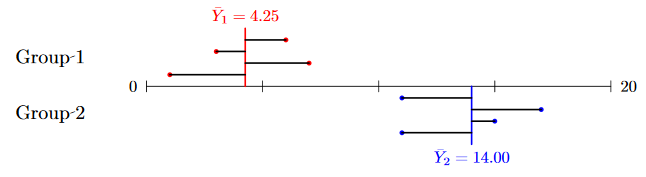
\includegraphics[width=\textwidth]{./chapters/2_statistics/05_common_statistical_tests/2_images/1_anova_inter_grp.PNG}
	\end{center}
	\caption{Deviations for within-group of squares}
	\label{fig:3_anovaInterGrp}
\end{figure}
\begin{center}
\fr{
$ MS_{within} = \dfrac{SS_{within}}{df_{within}}
\begin{cases}
	SS_{within} = \su{{j=1}}{k}SS_{j}=\su{{j=1}}{k}\su{{i=1}}{n_{j}}\left(Y_{ij}-\overline{Y}_{\bullet j}
	\right)\\
	df_{within} = df_{j} = \su{{j=1}}{k}(n_{j}-1) = N-k
\end{cases}
$
}\end{center}

\tB{$MS_{within}$ is a good estimate of $\sigma^{2}$ from our model regardless of the truth of 
$H_{0}$.} This is due to the way $SS_{within}$ is defined.

\begin{figure}[H]
	\begin{center}
		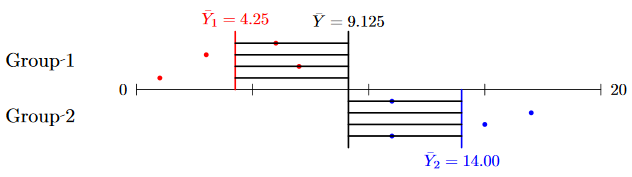
\includegraphics[width=\textwidth]{./chapters/2_statistics/05_common_statistical_tests/2_images/2_anova_btw.PNG}
	\end{center}
	\caption{Deviations for betwwen-group sum of squares}
	\label{fig:4_anovaBtw}
\end{figure}
$SS_{between}$ is the sum of the $N$ squared between-group deviations, where the deviation is
the same for all subjects in the same group. The formula is : 
\begin{center}
\fr{
$
MS_{Between} = \dfrac{SS_{Between}}{df_{between}}
\begin{cases}
SS_{between} = \su{{j=1}}{k}n_{j}\left(\overline{Y}_{\bullet j}-\overline{Y}\right)^{2}\\
df_{between} = k-1
\end{cases}
$
}\end{center}
Because of the way $SS_{between}$ is defined, \tB{$MS_{between}$ is a good estimate of $\sigma^{2}
$ only if $H_{0}$ is true}. Otherwise it tends to be larger. \\
The $F-statistic$ defined by $F=\dfrac{MS_{between}}{MS_{within}}$ \uR{tends to be larger if the
alternative hypothesis is true than if the null hypothesis is true}.\\

We can quantify ``large'' for the \emph{F-statistic}, by comparing it to its null sampling 
distribution which is the specific \emph{F-distribution}  which has degrees of freedom matching
the numerator and denominator of the \emph{F-statistic}.\\
Concerning inferences to build the confidence interval we need the \tB{\emph{standard error} (the
standard deviation of the means) that is $\sqrt{\dfrac{MS_{within}}{n_{i}}}$}\\
Let's detail the case where $p=2$ meaning comparison of  2 samples:
with means $\mu_{1}$ and $\mu_{2}$, and the same variance $\sigma^{2}$ and
finally $n=n_{1}+n_{2}$ observations.
Model: 
\begin{center}
	$\forall (j,i)\in\inter{1}{2}\times\inter{1}{n_{j}}y_{ij} = \mu_{j} + \epsilon_{ij} = \mu + \alpha_{j} + \epsilon_{ij}$
\end{center}
\uB{$\alpha_{j}=\mu_{j}-\mu$} is called (treatment-) effect

Decomposition:
\begin{align*}
	SS_{total} =& \su{{j=1}}{n_{1}}\left(y_{1j}-\overline{y}\right)^{2} +
	\su{{j=1}}{n_{2}}\left(y_{2j}-\overline{y}\right)^{2}\\
	=& \su{{j=1}}{n_{1}}\left(y_{1j}-\overline{y_{1}}+\overline{y_{1}}-\overline{y}\right)^{2}
	+ \su{{j=1}}{n_{2}}\left(y_{2j}-\overline{y_{2}}+\overline{y_{2}}-\overline{y}\right)^{2}\\
	=& \underbrace{(n_{1}-1)s_{1}^{2} + (n_{2}-1)s_{2}^{2}}_{SS_{within}} +
    \underbrace{n_{1}(\overline{y}_{1}-\overline{y})^{2} + 
	n_{2}(\overline{y}_{2}-\overline{y})^{2}}_{SS_{between}}
\end{align*}
\tB{$SS_{between}$ corresponds to squared enumerator $(\overline{y}_{1} - \overline{y}_{2})^{2}$ of
the statistic}: 
\begin{align*}
	SS_{between} =& n_{1}(\overline{y}_{1}-\overline{y})^{2} + 
	n_{2}(\overline{y}_{2}-\overline{y})^{2}\\
	=& n_{1}\left(\overline{y}_{1}-\dfrac{n_{1}\overline{y}_{1}+n_{2}\overline{y}_{2}}{n_{1}+
	n_{2}}\right)^{2} + n_{2}\left(\overline{y}_{2}-\dfrac{n_{1}\overline{y}_{1}+n_{2}
	\overline{y}_{2}}{n_{1}+ n_{2}}\right)^{2}\\
	=& \dfrac{n_{1}n_{2}}{n_{1}+n_{2}}\left(\overline{y}_{1}-\overline{y}_{2}\right)^{2}
\end{align*}
\tB{$SS_{within}$ corresponds to denominator of \emph{t-statistic}}:
$s=\sqrt{\dfrac{(n_{1}-1)s_{1}^{2}+(n_{2}-1)s_{2}^{2}}{n_{1}+n_{2}-2}}$\\
Pooled variance that is an estimate of the fixed common variance $\sigma^{2}$ underlying various
populations that have different means.
$\hat{\sigma}=\dfrac{(n_{1}-1)s_{1}^{2}+(n_{2}-1)s_{2}^{2}}{(n_{1}-1)+(n_{2}-1)}$\\
Null hypothesis $H_{0}:\mu_{1}=\mu_{2}$ or $\alpha_{1}=\alpha_{2}=0$ \\
\emph{F-test}
$\left(\overline{Y}_{1}-\overline{Y}_{2}\right)\hookrightarrow \mathcal{N}\left(\mu_{1}-\mu_{2},
\left(\frac{1}{n_{1}}+\frac{1}{n_{2}}\right)\sigma^{2}\right)\\
\E{\left[\overline{Y}_{1}-\overline{Y}_{2}\right]^{2}}=\left(\frac{1}{n_{1}}+\frac{1}{n_{2}}
\right)\sigma^{2}+(\mu_{1}-\mu_{2})^{2}\\
\E{MS_{between}}=\E{\frac{n_{1}n_{2}}{n_{1}+n_{2}}\left[\overline{Y}_{1}-\overline{Y}_{2}
\right]^{2}} = \sigma^{2}+\frac{n_{1}n_{2}}{n_{1}+n_{2}}(\mu_{1}-\mu_{2})^{2}\\
\E{MS_{whithin}}=\sigma^{2}\\
F = \dfrac{MS_{between}}{MS_{within}}$\\
Here $F=t^{2}$\\
\begin{align*}
	\text{Degrees of freedom} =& n - 1\\
	=& \underbrace{(n-m)}_{df_{within}} + \underbrace{(m-1)}_{df_{between}}
\end{align*}
\begin{itemize}
	\item $SS_{within}$ and $SS_{between}$ are independent
    \item \tB{under $H_{0}~\E{MS_{between}} = \E{MS_{within}} = \sigma^{2}$}
	\item \tB{under $H_{a}~\E{MS_{between}}>\sigma^{2}$ and $\E{MS_{within}} =
        \sigma^{2}$}
\end{itemize}
Hence $$ F= \dfrac{MS_{between}}{MS_{within}}\hookrightarrow F_{m-1,n-m}$$
In the case of 2 groups (``\emph{t-test}'') we received:
$$ \overline{y}_{1}-\overline{y}_{2} \pm t_{n-2,1-\frac{\alpha}{2}}s\sqrt{\frac{1}{n_{1}}+
\frac{1}{n_{2}}}$$


\paragraph{Assumptions}
The statistical model for which one-way ANOVA is appropriate is that the
\begin{itemize}
    \item (Quantitative) Outcomes for each group are normally distributed
    \item Outcome variances are all equal to  ($\sigma^{2}$)
    \item The errors are assumed to be independent.
\end{itemize}
\paragraph{Strengths}
\paragraph{Weaknesses}

\subsection{T-test}
It is commonly used when the test statistic would follow a normal distribution
if the value of a scaling term in the test statistic were known.\\
When the scaling term is estimated from the data, under certain conditions, the
test statistic follows a \emph{Student's t-test}.\\
Most test statistics have the form $t=\dfrac{Z}{s}$, $Z$ may be sensitive to 
the alternative hypothesis, whereas $s$ isa scaling parameter allowing to determine
the distribution \emph{t}.
\paragraph{One-sample}
$$
t = \dfrac{\overline{x} - \mu_{0}}{\frac{s}{\sqrt{n}}},
\begin{cases}
    \overline{x}\text{: sample mean}\\
    s\text{: sample standard deviation}\\
    n\text{: sample size}
\end{cases}
$$
By the central limit theorem, if the observations are independent and the second
moment exist, then $t$ will approximately follow the distribution $\mathcal{N}(0, 1)$

\paragraph{Assumptions}
Although the parent population does not need to be normally distributed, the distribution
of the population sample means $\left(\overline{x}_{s}\right)_{1\leq s\leq S}$.\\
\paragraph{Strengths}
\paragraph{Weaknesses}


\paragraph{Slope of a regression line}
Suppose one is fitting: $Y = \alpha + \beta x + \epsilon$, where $x$ is known and $\alpha$ and $\beta$ are unknown
and finally $\epsilon \hookrightarrow \mathcal{N(0, 1)}$.
Symbols with hat will refer to estimators.
\begin{center}
    \tB{$t_{score} = \dfrac{\hat{\beta} - \beta_{0}}{SE_{\hat{\beta}}} \hookrightarrow 
    \mathcal{T}_{n-2}$}
\end{center}
The standard error of the slope coefficient:
$\begin{cases}
    SE_{\hat{\beta}} &= \dfrac{\sqrt{\frac{1}{n-2}\su{i=1}{n}\left(y_{i}-
    \hat{y}_{i}\right)^{2}}}{
    \sqrt{\su{i=1}{n}\left(x_{i} - \overline{x}\right)^{2}}}\\
                SSR &= \su{i=1}{n}\hat{\epsilon}^{2}_{i} = \left(y_{i} - \hat{y}_{i}
                \right)
\end{cases}$

\paragraph{Independent 2-sample t-test}
\subparagraph{Equal sample sizes and variance}
$\begin{cases}
    t = \dfrac{\overline{X}_{1}-\overline{X}_{2}}{s_{p}\sqrt{\frac{2}{n}}} \\
    s_{p} = \sqrt{\dfrac{s_{X_{1}}^{2} + s_{X_{2}}^{2}}{2}}
\end{cases}$

\subparagraph{Unequal sample sizes and similar variances ($\frac{1}{2}<\frac{s_{X_{1}}}
{s_{X_{2}}}<2$)}:
$\begin{cases}
    t = \dfrac{\overline{X}_{1}-\overline{X}_{2}}{s_{p}\sqrt{\frac{1}{n_{1}} + 
    \frac{1}{n_{2}}}} \\
    s_{p} = \sqrt{\dfrac{(n_{1}-1)s_{X_{1}}^{2} + (n_{2}-1)s_{X_{2}}^{2}}{n_{1} + n_{2}
    -2}}
\end{cases}$

\subparagraph{Unequal sample sizes and unequal variances ($s_{X_{1}} > 2s_{X_{2}}$ 
or $s_{X_{2}} > 2s_{X_{1}}$)}:
$\begin{cases}
    t = \dfrac{\overline{X}_{1}-\overline{X}_{2}}{s_{\Delta}} \\
    s_{\Delta} = \sqrt{\dfrac{s_{X_{1}}^{2}}{n_{1}}+\dfrac{s_{X_{2}}^{2}}{n_{2}}}
\end{cases}$

\paragraph{Dependent t-test for paired samples}
$t=\dfrac{\overline{X}_{D} - \mu_{0}}{\frac{s_{D}}{\sqrt{n}}}$
\paragraph{Assumptions}
\paragraph{Strengths}
\paragraph{Weaknesses}
